\documentclass{../download/tPRS2e}

\usepackage{epstopdf}% To incorporate .eps illustrations using PDFLaTeX, etc.
\usepackage{subfigure}% Support for small, `sub' figures and tables

\graphicspath{{media/}}

\begin{document}

\title{About some types of constraints in problems of routing}

\author{
\name{
Petunin A.A.\textsuperscript{a},
Polishuk E.G.\textsuperscript{a},
Chentsov A.G.\textsuperscript{b}\textsuperscript{a},
Chentsov P.A.\textsuperscript{a}\textsuperscript{b},
Ukolov S.S.\textsuperscript{a}$^{\ast}$\thanks{$^\ast$Corresponding author. Email: s.s.ukolov@urfu.ru}
}
\affil{\textsuperscript{a}Ural Federal University, Yekaterinburg, Russia;
\textsuperscript{b}Institute of Mathematics and Mechanics, Ural Branch of the Russian Academy of Sciences, Yekaterinburg, Russia}
}

\maketitle

\begin{abstract}
Many routing problems arising in different applications can be interpreted
as a discrete optimization problem with additional constraints.
The latter include generalized travelling salesman problem (GTSP),
to which task of tool routing for CNC thermal cutting machines is sometimes reduced.
Technological requirements bound to thermal fields distribution during cutting process
are of great importance when developing algorithms for this task solution.
These requirements give rise to some specific constraints for GTSP.
This paper provides a mathematical formulation for the problem of
thermal fields calculating during metal sheet thermal cutting.
Corresponding algorithm with its programmatic implementation is considered.
The mathematical model allowing taking such constraints into account
considering other routing problems is discussed either. 
\end{abstract}

\begin{keywords}
thermal cutting;
discrete optimization;
toolpath routing;
technological constraints;
dynamic programming;
thermal deformations
\end{keywords}

\section{Introduction}

In various industries many parts are produced from sheet materials by CNC equipment.
Such kind of equipment includes, for instance, machines for laser, plasma, gas, and water-jet cutting.
Special software (Computer-Aided Manufacturing, CAM systems) provides an automation of development of NC (numerical control) programs.
Generating of NC programs is next step after nesting that is positioning parts onto sheet material.
Optimization of sheet utilization reduces the cost of sheet material used for parts producing.
The nesting problem is not considered in this study.
The control programs contain information about tool path for CNC machine and some technological commands.
Optimization of tool path reduces time and cost of cutting process.
First classification of problem was conducted by \cite{hoeft_heuristics_1997}. 
Tool path problems are usually divided into 4 classes depending on cutting technique and its parameters (see, for example, \cite{dewil_improvement_2015}):

\begin{enumerate}
\item \textit{Continuous Cutting Problem (CCP)}.
\item \textit{Endpoint Cutting Problem (ECP)}.
\item \textit{Intermittent Cutting Problem (ICP)}. 
\item \textit{Generalized Traveling Salesman Problem (GTSP)}.
\end{enumerate}

\cite{petunin_modeling_2015} offered new classification of cutting techniques and described one more class of problem:
\textit{Segment Continuous Cutting Problem (SCCP)}.

\subsection{Tool Path Components}

The tool path contains the following components (see Fig.\ref{toolpath}):

\begin{itemize}
\item Pierce points (piercings);
\item Points of switching the tool off;
\item Tool trajectory from piercing up to point of switching the tool off; 
\item Lead-in (tool trajectory from piercing up to the entry point on the equidistant contours); 
\item Lead-out (tool trajectory from exit point on equidistant contour up to tool switching off point); 
\item Airtime motions (linear movement from tool switching off point up to the next piercing).
\end{itemize}

\begin{figure}
\begin{center}
\includegraphics[width=0.6\textwidth]{toolpath.pdf}
\caption{Scheme of the standard cutting technique.} \label{toolpath}
\end{center}
\end{figure}


\subsection{Cutting Techniques}

All the cutting techniques can be divided into three classes:

\begin{enumerate}
\item Standard cutting. 
\item Multi-contour cutting.
\item Multi-segment cutting.
\end{enumerate}

Standard cutting technique assumes:

\begin{itemize}
\item Piercings number is equal to contours number and parts number;
\item Cutter head runs each closed equidistant contour of part to cut exactly once from beginning to end. 
\end{itemize}

The multi-contour cutting cuts several contours in one segment of cutting.
External contours of parts are cut jointly with the only piercing without switching cutter head off.
Multi-segment cutting cuts single contour in several segments of cutting (see Fig. \ref{???}).

\section{Formal Definition of Tool Path}

Let $A_1, A_2, \dots A_n$ to be finite set of two-dimensional geometrical objects
(representations of parts to cut).
Each object is described by one or several closed curves (boundary contours). 
Let also $N$ to be number of external and the internal closed contours $C_1, C_2, \dots C_N$,
that describe parts positions (the nesting) on sheet material
$(A_i, C_j \subset \mathbb{R}^2; i = \overline{1,n}, j = \overline{1, N}, j \ge n )$.

We define cutting segment  $S = \overrightarrow{M B^S M^*}$
as a tool trajectory from piercing  $M$ up to point of switching the tool off  $M^*$
$(S \subset \mathbb{R}^2; M = (x, y), M^ *= (x^*, y^*) \in \mathbb{R}^2)$.
Basic segment $B^S$ is a part of segment $S = \overrightarrow{M M^*}$
without trajectory lead-in and trajectory lead-out.

Unlike full segment (which is oriented),
its basic segment can be cut in both directions,
it contains only geometric information.

Let $K$ be the number of segments the tool path consists of.
$S_k = \overrightarrow{M_k M_k^*}; k = \overline{1, K}$.
Single segment may contain one contour,
a few contours (for the multi-contour cutting),
or a part of contour (for multi-segment cutting).
Sequence of segments is a permutation $i_1, i_2, \dots, i_K$,
i.e. the ordered set of natural numbers from $1$ to $K$
or bijection on a set $\{\overline{1, K}\}$.

Finally, the tool path is defined by a tuple:

\begin{equation} \label {tuple}
ROUTE = < S_1, S_2, \dots S_K, i_1, i_2, \dots i_K > 
\end{equation}

During development of NC programs for CNC sheet metal cutting machines the problems of tool path optimization arise.
As optimization criteria in these problems the parameters of cutting time $t_{cut}$ and cost $F_{cost}$ are considered.
They are calculated by following formulas:

\begin{equation} \label{time}
t_{cut} = L_{on} \div V_{on} + L_{off} \div V_{off} + N_{pt} \cdot t_{pt}
\end{equation}

\begin{equation} \label {cost}
F_{cost} = L_{on} \cdot C_{on} + L_{off} \cdot V_{off} + N_{pt} \cdot C_{pt}
\end{equation}

Here $L_{off}$ is length of idling tool path;
$L_{on}$ is length of working tool path;
$V_{off}$ is speed of idling tool path;
$V_{on}$ is speed of the working tool path;
$C_{off}$ is cost of idling tool path unit;
$C_{on}$ is cost of working tool path unit;
$N_{pt}$ is numbers of piercing;
$t_{pt}$ is time of one piercing;
$C_{pt}$ is cost of one piercing.

Objective functions (\ref{time}) and (\ref{cost})
for the tool path depend on elements of tuple (\ref{tuple}).
Let us consider technological constraints on tuple
$<M_1, M_1^*, \dots , M_K, M_K^*, i_1, \dots , i_K>$
elements.

\section{Tool Path Constraints Formalization}

As we mentioned above,
the tool path routing problem is often reduced to the Generalized Traveling Salesman Problem (GTSP),
since a lot of algorithms are known to exist to solve it.
Unfortunately, most solutions are not feasible for tool path routing problem due to many technological restrictions,
especially dealing with thermal deformations during cutting process.
These restrictions are mostly empirical,
but after mathematical formalization they impose some strict constraints on the elements of tuple (\ref{tuple}).
In some cases these constraints can be used to significantly reduce dimension of problem space,
leading to decreasing computation complexity.

\subsection{Precedence Constraint}

For most CNC cutting machines when some part (bounded with a closed contour) has been cut,
nothing prevents it from slightly moving on the cutting table.
Therefore, one cannot reliably cut inner contours (holes) of that part.
This also applies to other parts, positioned in the holes of the former one.

This constraint is well known and described in many papers
(e.g. \cite{verkhoturov_mathematical_2008}, 
\cite{dewil_cutting_2011})
Its formalization and implementation usually doesn’t meet with great difficulties.

In terms of tuple (\ref{tuple}),
this constraint imposes restrictions on permutation 
$I = \{i_1, i_2, \dots i_K\}$.
\cite{petunin_2014}
showed that this reduction of feasible permutations allows some algorithms that get exact solutions for some problems of big dimension.

\subsection{Piercing Coordinates Constraints}

This constraint is due to another technological feature of sheet cutting.
Material deformation in the beginning of cutting segment (point of piercing) is usually greater than in its other points.
So, the piercing point must lay at event greater distance from part boundary than cutting itself.
Exact values of these two distances depend on technological parameters.
In terms of tuple (\ref{tuple}) this constraints narrows the choice of feasible piercing points $M_i$
for every segment $S_i$. (see Fig. \ref{piercing-area})

Let us denote as $E^d_j (j = \overline{1, N})$
an equidistant contour for part boundary $C_j$
offset with a distance d:
$E^d_j \subset \mathbb{R}^2$.
$P^d_j$ is two-dimensional shape, bounded by $E^d_j (j=\overline{1, N})$.

Next, let $OUT$ is a set of external contours indexes,
while $IN$ is a set of internal contours indexes,
i.e. $OUT \subseteq \{\overline{1, N}\},  IN \subseteq \{\overline{1, N}\}$.
When $N = n$, all contours are external $OUT=\{\overline{1, N}\}, IN = \varnothing$.

Let $\partial$  is a half width (a half allowance) for the cutting process.
Then trajectories of the cutting segments for cutting of parts $A_1, A_2, \dots A_n$ has to contain all contours  $E^\partial_j (j = \overline{1, N})$:
$$
\bigcup^N_{j=1} E^\partial_j
\subseteq
\bigcup^K_{k=1} B^{S_k}
\subset
\bigcup^K_{k=1} S_k
$$

Let $\delta$  is a minimal distance from piercing point to equidistant contour (defined by technology).
Then piercing points and tool switching off points must meet the following conditions (see Fig. \ref{piercing-area}):

\begin{equation} \label{on-point}
M_k \in
( B \backslash \bigcup_{j \in OUT} P^{\partial + \delta}_j ) \bigcup_{q \in IN} P^{\partial + \delta}_q
\end{equation}

\begin{equation} \label{off-point}
M_k^* \in
( B \backslash \bigcup_{j \in OUT} P^\partial_j ) \bigcup_{q \in IN} P^\partial_q
\end{equation}

Having all feasible positions for piercing points $M_i$ found,
one can reduce full tool path optimization problem
(which is both continuous and discrete optimization problem)
to discrete one simply by selecting finite set of possible piercing points on the border of area,
defined by (\ref{on-point}), see Fig. \ref{discrete}.

\begin{figure}
\begin{center}
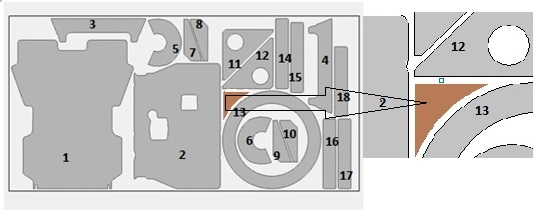
\includegraphics[width=\textwidth]{ppc.jpeg}
\caption{Feasible piercing area is marked with brown color.} \label{piercing-area}
\end{center}
\end{figure}

\begin{figure}
\begin{center}
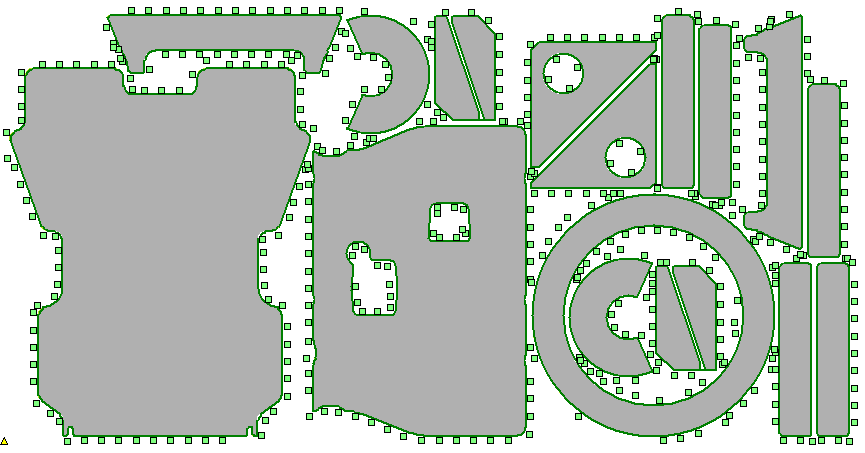
\includegraphics[width=0.6\textwidth]{discrete.png}
\caption{Example of finite set of piercing points.} \label{discrete}
\end{center}
\end{figure}


\subsection{Part Hardness Rule}

\subsubsection{Formalization of Part Hardness Rule}

\subsubsection{Thermal Distribution Calculations}

A series of numerical experiments was conducted to better understand a nature of Part Hardness Rule.
For predefined sheet size, nesting, beam radius and power and cutting speed thermal filed was directly calculated using:

These calculations can be also used as another (or additional) considerations for selecting piercing points and cutting directions.
So far it is not practical though, for it takes too much time to calculate the whole thermal distribution for all the cutting process.
More investigations in this direction are necessary.

\subsection{Sheet Hardness Rules}

As well as Part Hardness Rule, this series of constraints is to minimize thermal deformations during thermal cutting process.
Unlike the former it primarily deals with second part (permutation) of tuple (\ref{tuple}).
It defines sequence of parts cutting. It is also mainly empirical.

The following rules are known:

\begin{itemize}
\item Start from sheet short edge
\item Long narrow parts, located next to sheet edge should be cut first
\item If a big free area (having no parts nested) exists, cutting should start from opposite sheet side
\item Start from the side with greater heat release (smaller parts or greater total perimeter)
\item Avoid uncut “islands”
\item Avoid long narrow uncut areas
\end{itemize}

\section{Discrete Optimization Algorithms}

\begin{figure}
\begin{center}
\subfigure[Exact SCCP solution.]{
\resizebox*{0.4\textwidth}{!}{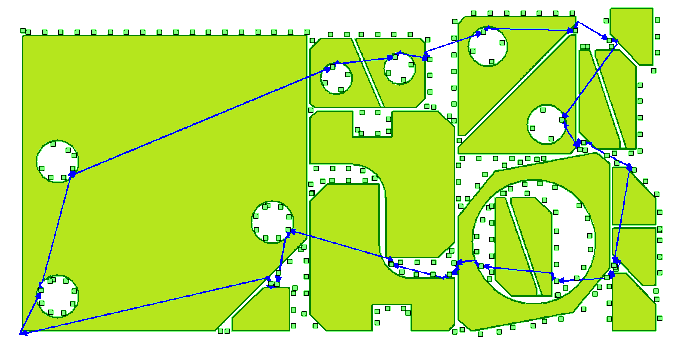
\includegraphics{nest-a.png}}}
\subfigure[Solution with thermal cutting constraints.]{
\resizebox*{0.4\textwidth}{!}{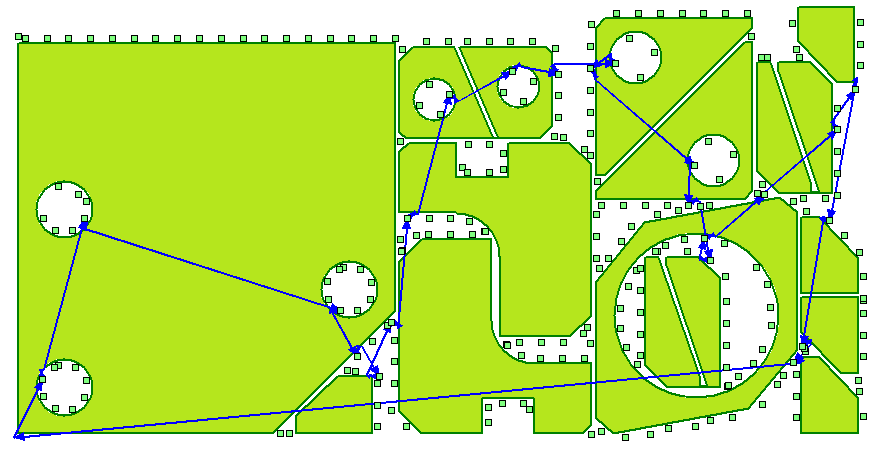
\includegraphics{nest-b.png}}}
\caption{Results of tool path optimizations.} \label{nesting-results}
\end{center}
\end{figure}

See Fig. \ref{nesting-results}...

\section*{Acknowledgements}

The work was supported by Act 211 Government of the Russian Federation, contract № 02.A03.21.0006

\bibliographystyle{../download/tPRS}
\nocite{*}
\bibliography{Investigation}



\end{document}
